% Power electronics---the schematic diagram of a solar system connected to the grid.
% Author: Ali Mehrizi-Sani
\documentclass{standalone}

\usepackage[usenames,dvipsnames]{color}
\usepackage[american,cuteinductors,smartlabels]{circuitikz}
%%%<
\usepackage{verbatim}
%%%>
\begin{comment}
:Title: Power electronics - The schematic diagram of a solar system connected to the grid
:Tags: coordinate calculations;circuitikz;physics;electrical engineering
:Author: Ali Mehrizi-Sani
:Slug: power-electronics-solar-system
\end{comment}
\usepackage{siunitx}
\usepackage{amsmath,amssymb}

\usetikzlibrary{calc}
\usetikzlibrary{patterns}
\ctikzset{bipoles/thickness=1}
\ctikzset{bipoles/length=0.8cm}
\ctikzset{bipoles/diode/height=.375}
\ctikzset{bipoles/diode/width=.3}
\ctikzset{tripoles/thyristor/height=.8}
\ctikzset{tripoles/thyristor/width=1}
\ctikzset{bipoles/vsourceam/height/.initial=.7}
\ctikzset{bipoles/vsourceam/width/.initial=.7}
\tikzstyle{every node}=[font=\small]
\tikzstyle{every path}=[line width=0.8pt,line cap=round,line join=round]

\definecolor{AleeRed}{rgb}{0.5,0,0}

\begin{document}

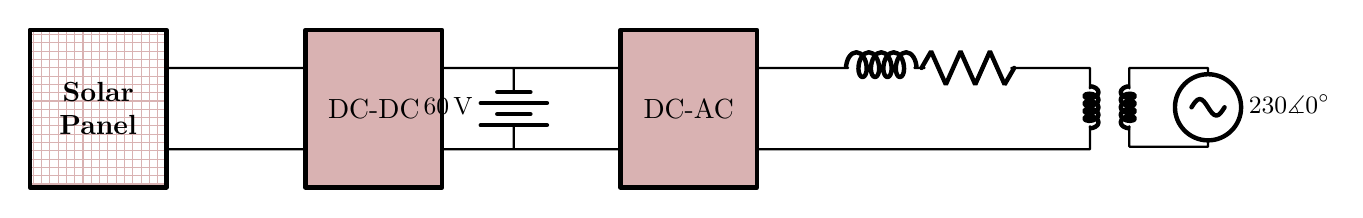
\begin{tikzpicture}
    \coordinate (SolarCellP) at (0.5,0);
    \coordinate (ChopperP) at (4,0);
    \coordinate (InverterP) at (8,0);

    % Place blocks
    \begin{scope}[every node/.style={draw,ultra thick, fill=AleeRed!30, rectangle,text width=1.5cm, minimum height=2cm, text badly centered}]
        \node[name=pv,pattern=grid,pattern color=AleeRed!30] at (SolarCellP) {\bfseries Solar Panel};
        \node[name=chopper] at (ChopperP) {DC-DC};
        \node[name=inverter] at (InverterP) {DC-AC};
    \end{scope}

    \draw
    % PV to chopper
        (pv.30) -- (chopper.150)
        (pv.330) -- (chopper.210)
    % DC link and cap
        (chopper.30) -- (inverter.150)
        (chopper.330) -- (inverter.210)
        ($(chopper.330)!0.4!(inverter.210)$) to[battery, l=\SI{60}{\volt}, mirror] ($(chopper.30)!0.4!(inverter.150)$)
    % AC side
        (inverter.30)
        to[short] ++(1,0)
        to[L] ++(1.1,0)
        to[R] ++(1.1,0)
        to[short] ++(1,0) coordinate(N1)
        to[L, bipoles/length=0.8cm] ++(0,-1)
        |- (inverter.330)
        % ------------------------ Secondary side
        (N1)++(0.5,0) coordinate (N2)
            to[open] ($(N2)+(0,-1)$)
            to[L, bipoles/length=0.8cm] (N2)
            to[short] ++(1,0)
            to[sV, l=$230\measuredangle 0^\circ$] ++(0,-1)
            to[short] ++(-1,0)
    ;
\end{tikzpicture}

\end{document} 